\documentclass[a4paper,11pt]{article}

\usepackage[left=2.5cm,right=2.5cm,top=3cm,bottom=3cm,pdftex]{geometry}
\usepackage{amssymb, amsmath, url, natbib, float, subcaption, listings,mathtools}
\usepackage[utf8]{inputenc}
\usepackage[T1]{fontenc}
\renewcommand{\topfraction}{0.9}
\lstset{basicstyle=\scriptsize\tt,}
\usepackage[pdftex]{graphicx}
\pdfcompresslevel=9 
\DeclareGraphicsExtensions{.png, .pdf, .jpg}
\usepackage[pdftex, colorlinks, linkcolor=blue, urlcolor=blue, citecolor=blue, pagecolor=blue, breaklinks=true]{hyperref}

\begin{document}
\pagestyle{empty}
\title{Comparison - pomp}
\begin{center}
\Large\textbf{POMP results} \\[11pt]
\normalsize
\end{center}

\begin{table}[H]
\centering
\caption{pomp table}
\begin{tabular}{|l|l|l|l|}
\hline
POMP dt & Mean & Std Dev    & AR Rate \\ \hline
     & 0.959 & 0.058 & 10.99           \\
by2  & 0.808 & 0.123  &                 \\
     & 4.014  & 0.076 &                 \\ \hline
     & 1.003  & 0.083 & 16.41           \\
by4  & 0.953 & 0.125   &                 \\
     & 3.991  & 0.367  &                 \\ \hline
     & 1.009  & 0.047   & 17.13           \\
by8  & 1.012  & 0.098 &                 \\
     & 4.022  & 0.087 &                 \\ \hline
\end{tabular}
\end{table}

\begin{table}[H]
\centering
\caption{Comparing results of pomp and dtq}
\begin{tabular}{|ll|c|c|c|l|l|l|l|l|}
\hline
                                 &          &        & Mean   &        & RMS &        & Std Dev &        & Accept \\ \cline{3-5} \cline{7-9}
                                 &          & $\theta_1$ & $\theta_2$ & $\theta_3$ & error & $\theta_1$ & $\theta_2$  & $\theta_3$ & rate (\%)  \\ \hline
\multicolumn{1}{|l|}{h = 0.1}    & Eulerian & 0.747  & 0.906  & 3.072  & 0.557     & 0.062  & 0.076   & 0.031  & 29.55   \\ \hline
\multicolumn{1}{|l|}{h = 0.05}   & pomp     & 0.960  & 0.809  & 4.014  & 0.113     & 0.058  & 0.123   & 0.076  & 10.99   \\ \cline{2-10} 
\multicolumn{1}{|l|}{}           & dtq      & 0.866  & 1.305  & 4.260  & 0.244     & 0.043  & 0.082   & 0.092  & 28.53   \\ \hline
\multicolumn{1}{|l|}{h = 0.025}  & pomp     & 1.004  & 0.954  & 3.992  & 0.027     & 0.083  & 0.125   & 0.367  & 16.41   \\ \cline{2-10} 
\multicolumn{1}{|l|}{}           & dtq      & 0.892  & 1.157  & 4.430  & 0.271     & 0.048  & 0.069   & 0.037  & 25.43   \\ \hline
\multicolumn{1}{|l|}{h = 0.0125} & pomp     & 1.01   & 1.01   & 4.02   & 0.015     & 0.048  & 0.098   & 0.087  & 17.14   \\ \cline{2-10} 
\multicolumn{1}{|l|}{}           & dtq      & 0.98   & 1.17   & 4.21   & 0.155     & 0.039  & 0.077   & 0.035  & 23.87   \\ \hline
\end{tabular}
\end{table}

\begin{figure}[H]
\begin{subfigure}{0.48\textwidth}
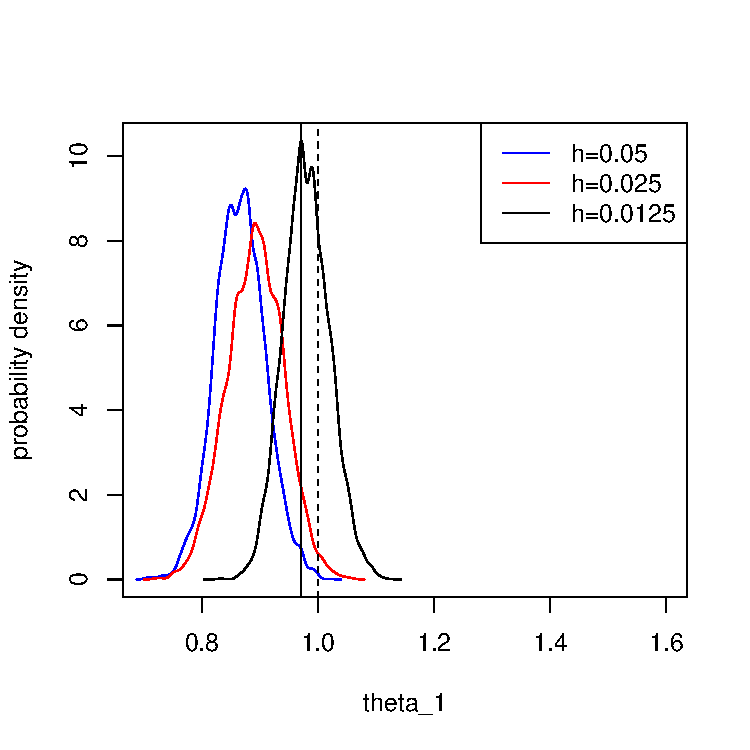
\includegraphics[width=\linewidth]{dtq_theta1.pdf}
\caption{$\theta_1$ for DTQ} \label{fig:a}
\end{subfigure}\hspace*{\fill}
\begin{subfigure}{0.48\textwidth}
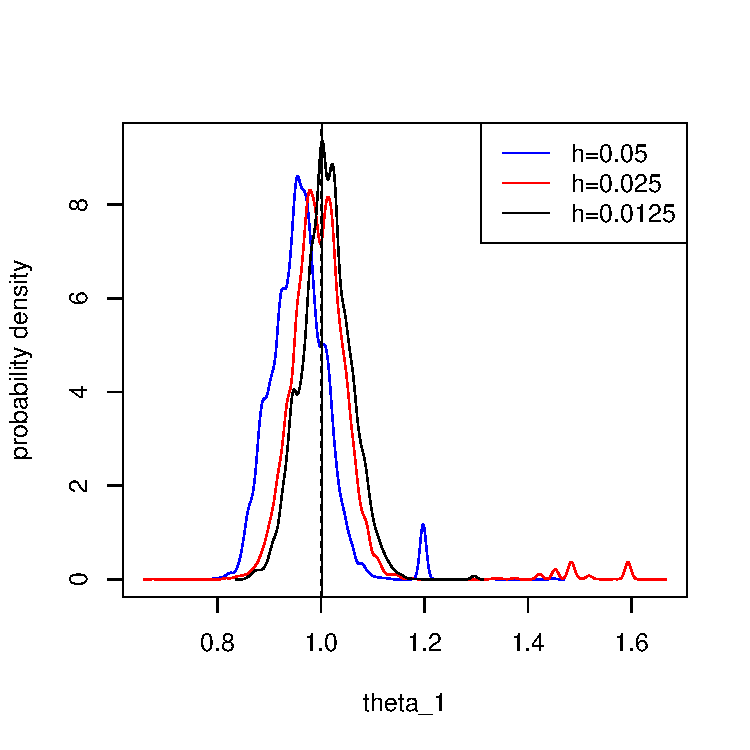
\includegraphics[width=\linewidth]{pomp_theta1.pdf}
\caption{$\theta_1$ for POMP} \label{fig:b}
\end{subfigure}

\medskip
\begin{subfigure}{0.48\textwidth}
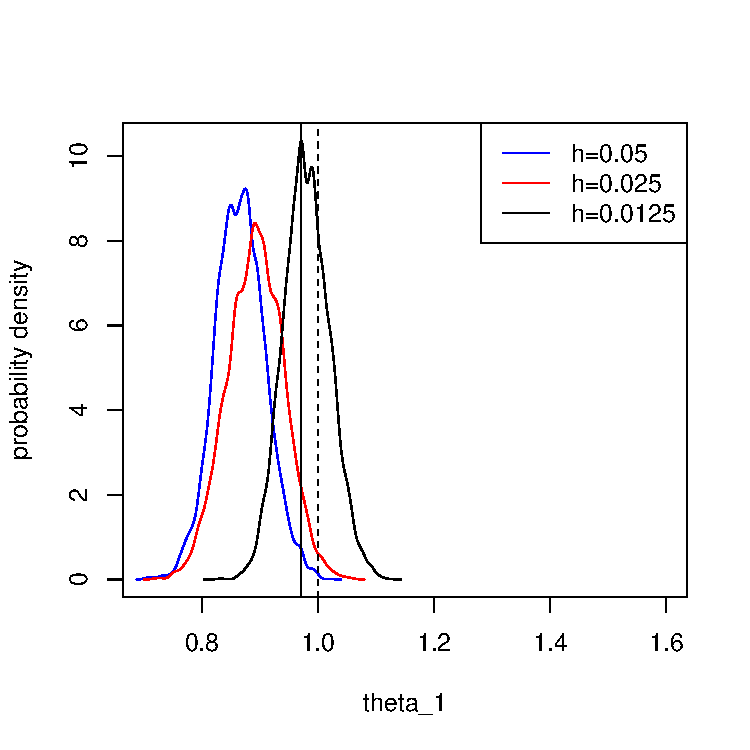
\includegraphics[width=\linewidth]{dtq_theta2.pdf}
\caption{$\theta_2$ for DTQ} \label{fig:c}
\end{subfigure}\hspace*{\fill}
\begin{subfigure}{0.48\textwidth}
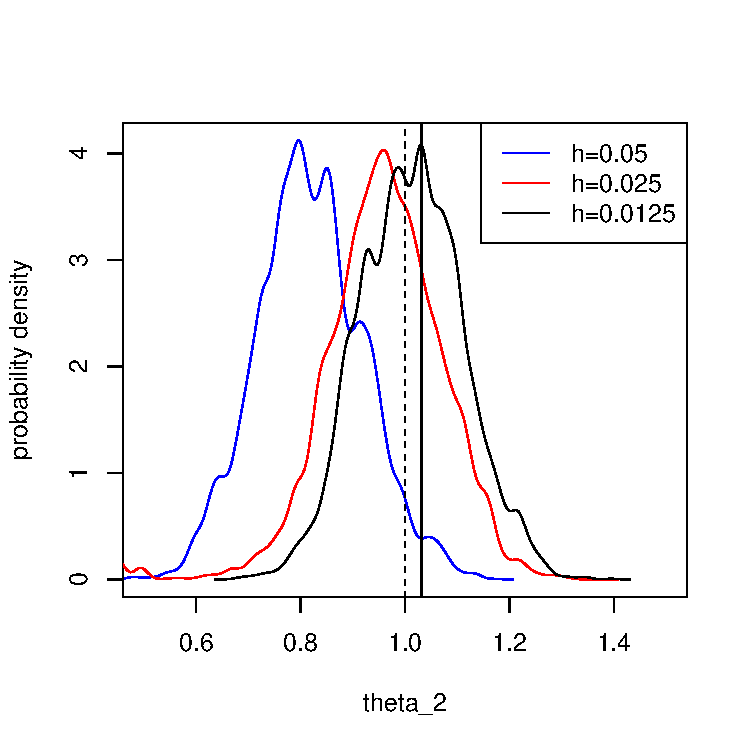
\includegraphics[width=\linewidth]{pomp_theta2.pdf}
\caption{$\theta_2$ for POMP} \label{fig:d}
\end{subfigure}

\medskip
\begin{subfigure}{0.48\textwidth}
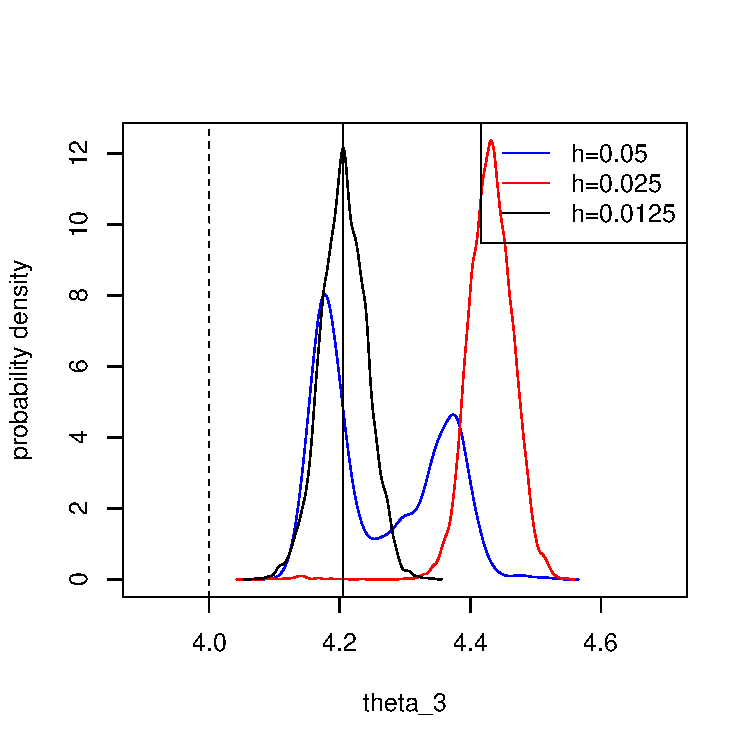
\includegraphics[width=\linewidth]{dtq_theta3.pdf}
\caption{$\theta_3$ for DTQ} \label{fig:e}
\end{subfigure}\hspace*{\fill}
\begin{subfigure}{0.48\textwidth}
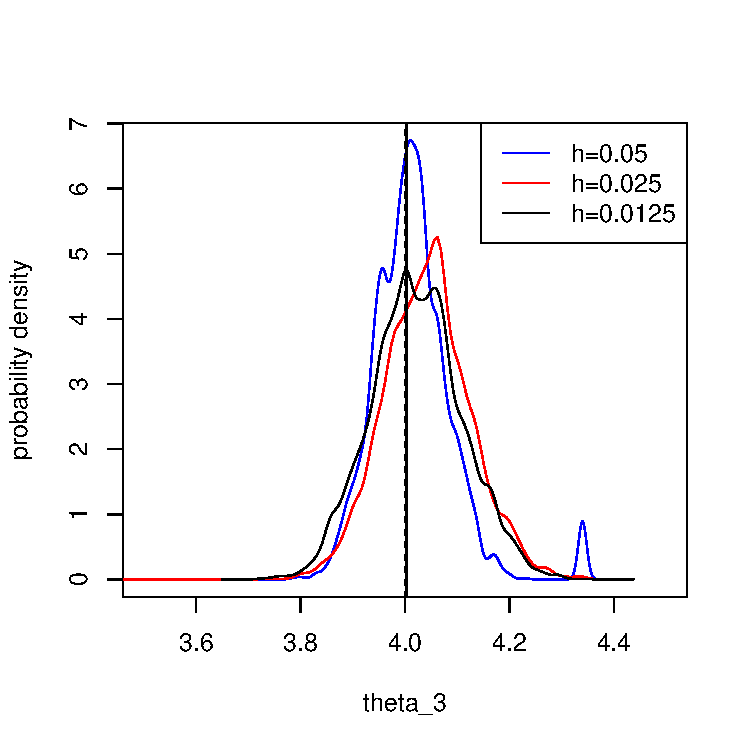
\includegraphics[width=\linewidth]{pomp_theta3.pdf}
\caption{$\theta_3$ for POMP} \label{fig:f}
\end{subfigure}

\caption{Probability density comparison plots for DTQ and POMP for varying time steps ($h = 0.05, 0.025, 0.0125$).} \label{fig:1}
\end{figure}
 
\newpage

\begin{figure}[H]
\begin{subfigure}{0.48\textwidth}
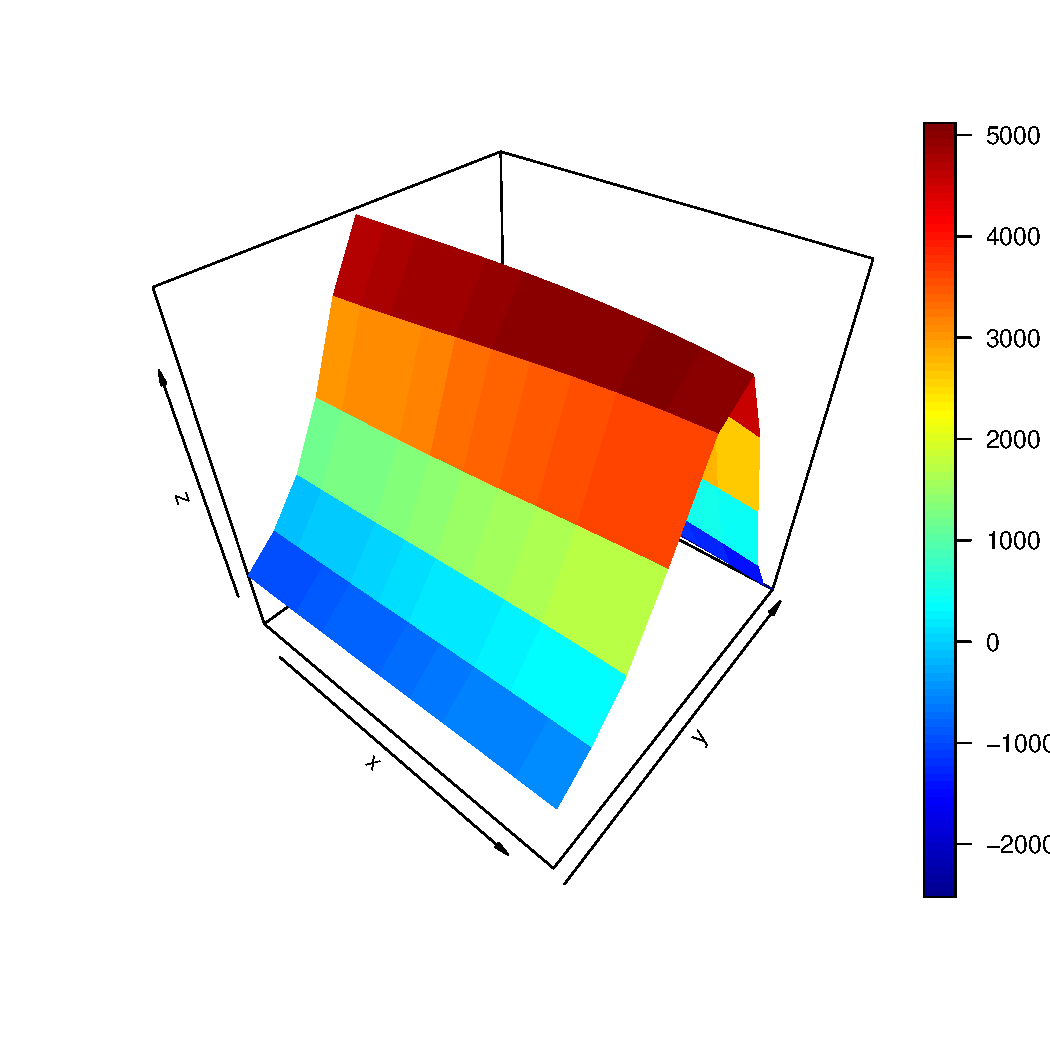
\includegraphics[width=\linewidth]{dtq_by10_by2.pdf}
\caption{DTQ by 100, by 2} \label{fig:a}
\end{subfigure}\hspace*{\fill}
\begin{subfigure}{0.48\textwidth}
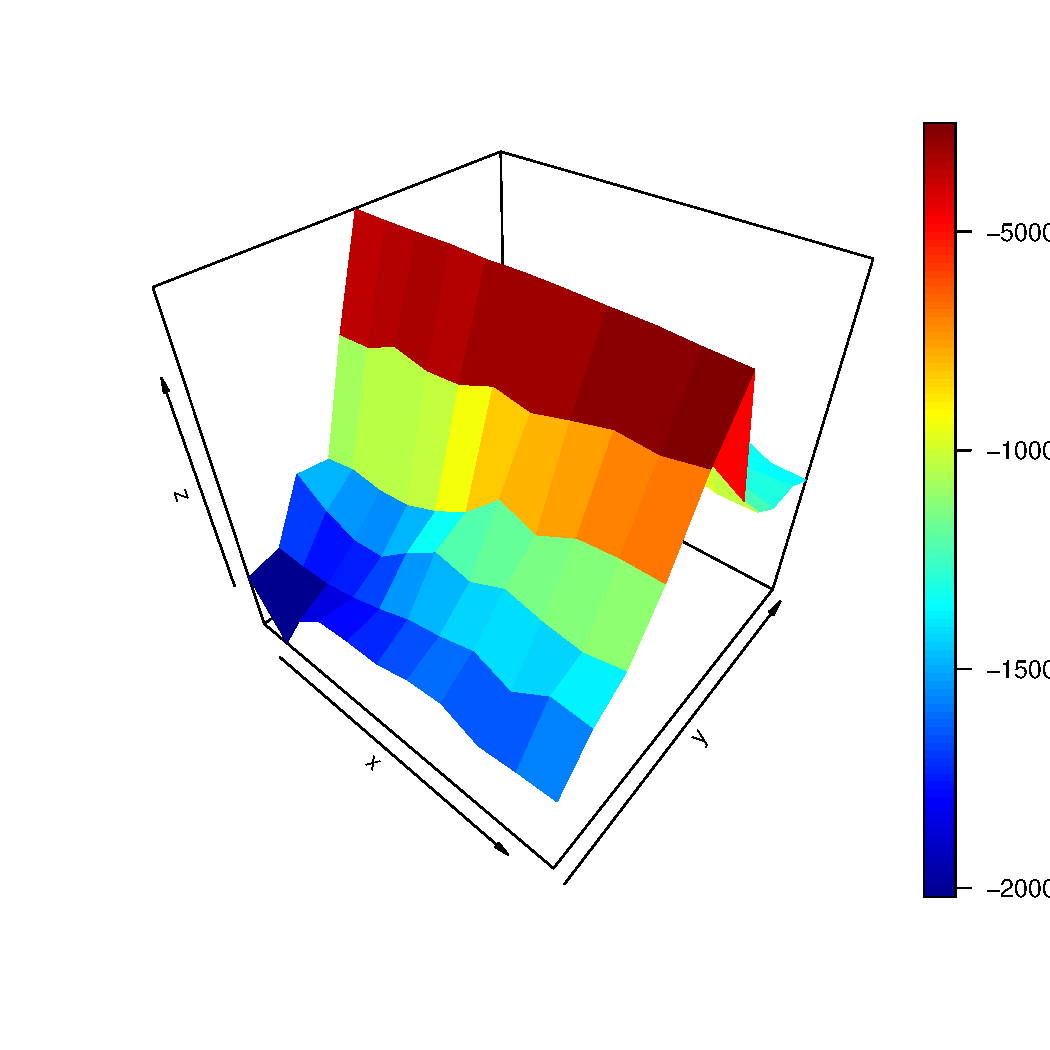
\includegraphics[width=\linewidth]{pomp_by10_by2.pdf}
\caption{POMP by 100, by 2} \label{fig:b}
\end{subfigure}

\medskip

\begin{subfigure}{0.48\textwidth}
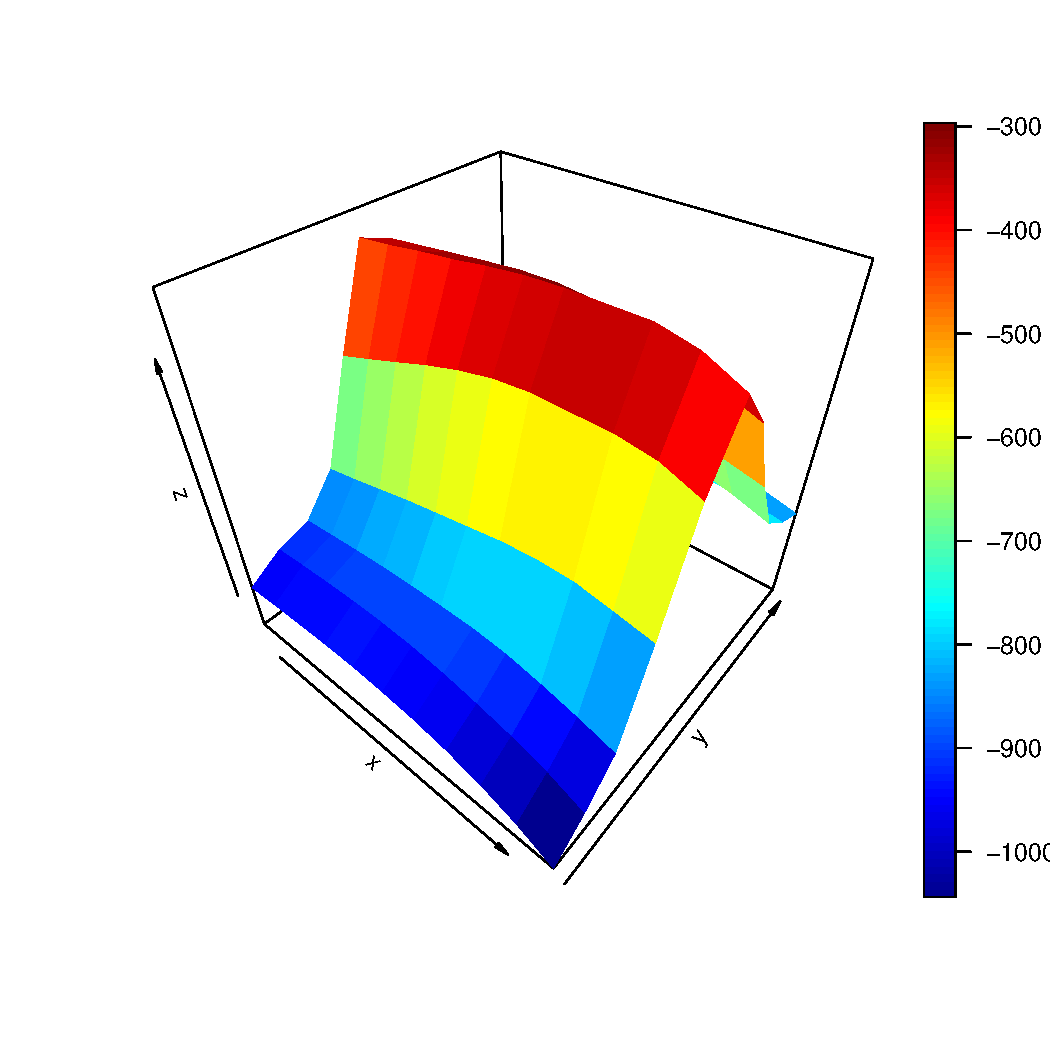
\includegraphics[width=\linewidth]{dtq_by100_by2.pdf}
\caption{DTQ by 100, by 2} \label{fig:a}
\end{subfigure}\hspace*{\fill}
\begin{subfigure}{0.48\textwidth}
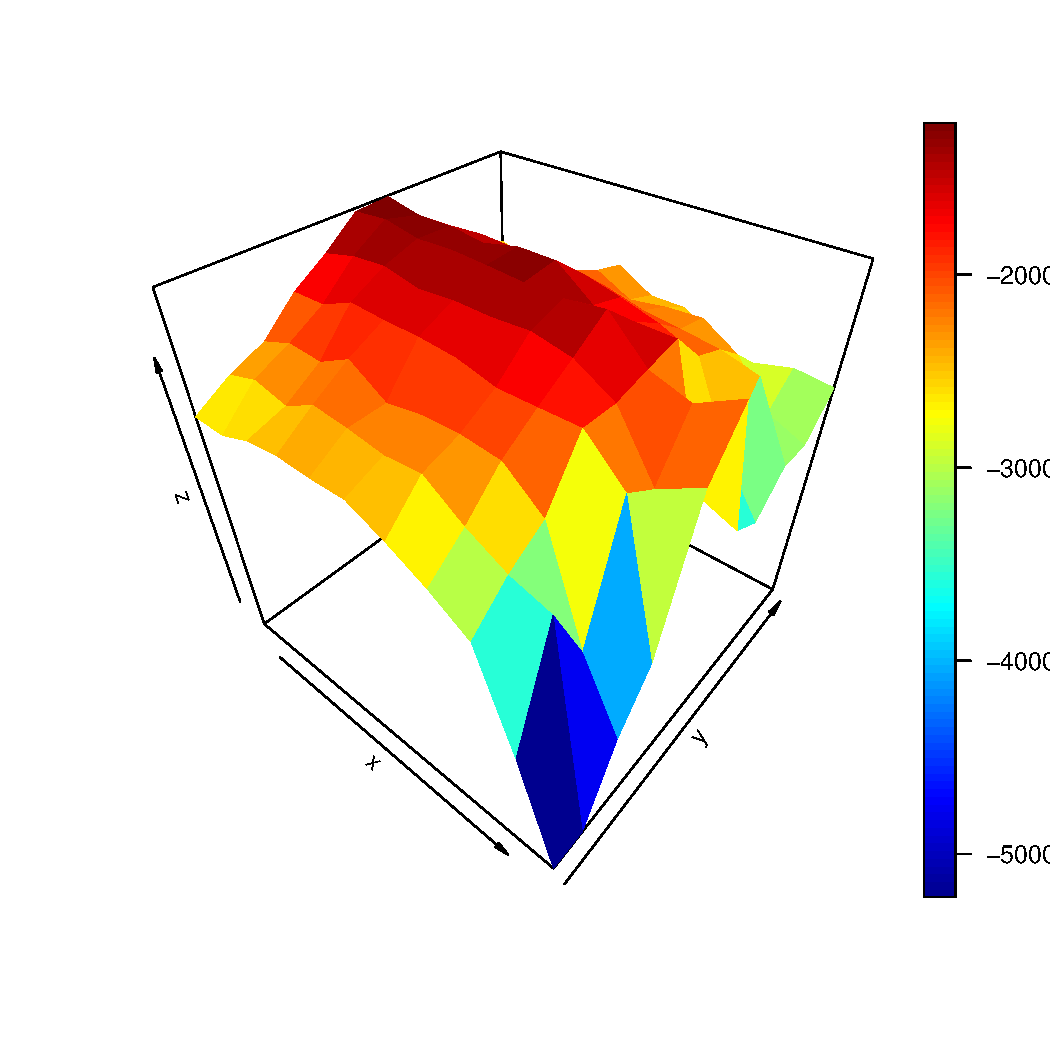
\includegraphics[width=\linewidth]{pomp_by100_by2.pdf}
\caption{POMP by 100, by 2} \label{fig:b}
\end{subfigure}

\medskip

% \begin{subfigure}{0.48\textwidth}
% 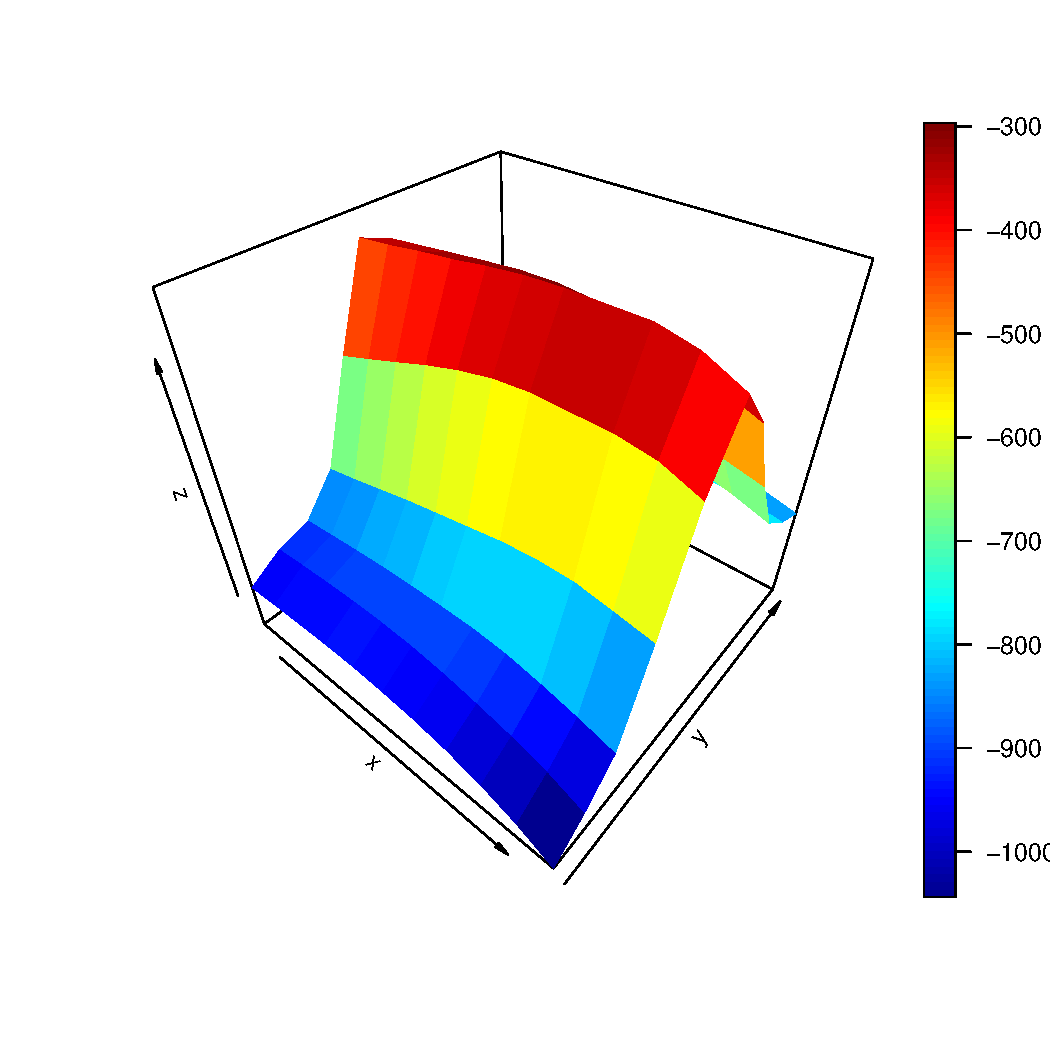
\includegraphics[width=\linewidth]{dtq_by100_by8.pdf}
% \caption{DTQ by 100, by 8} \label{fig:c}
% \end{subfigure}\hspace*{\fill}
% \begin{subfigure}{0.48\textwidth}
% 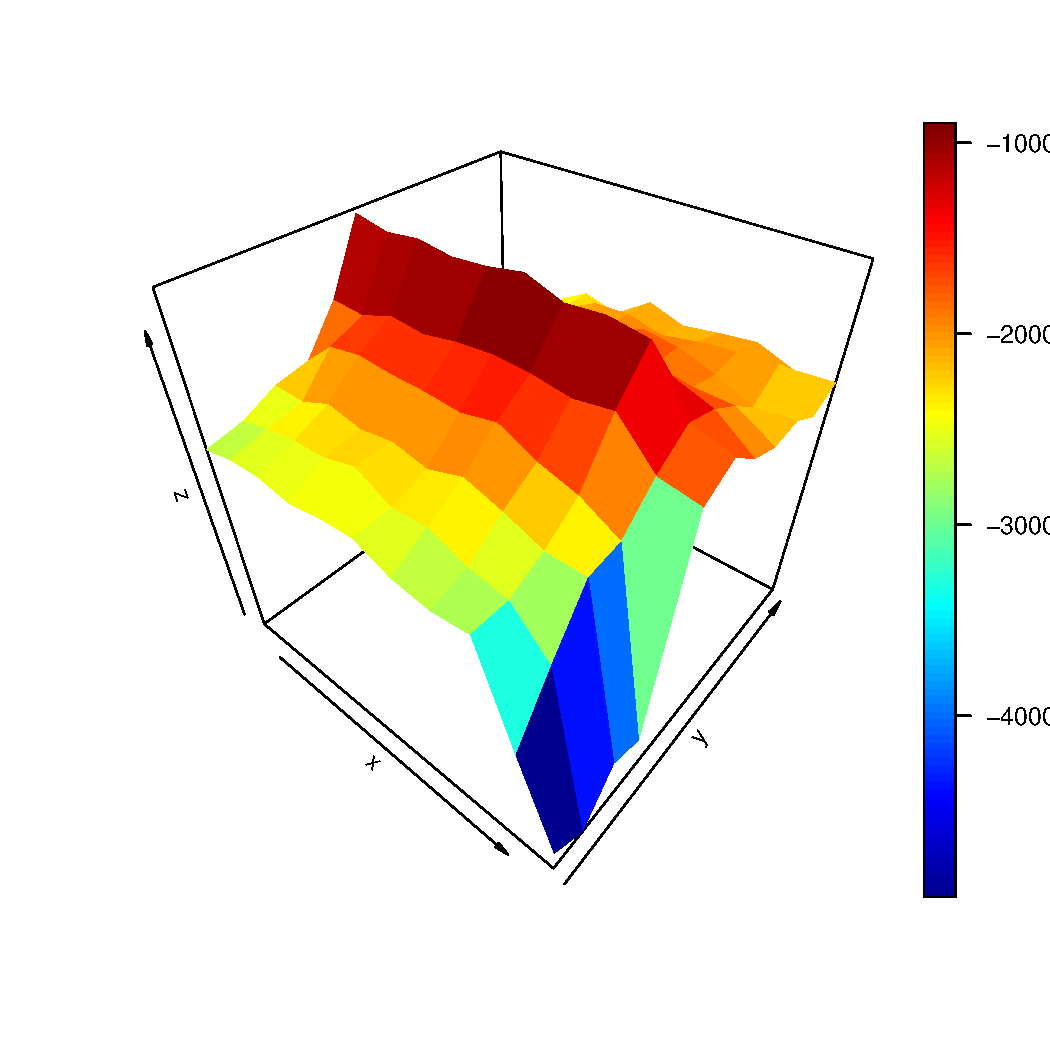
\includegraphics[width=\linewidth]{pomp_by100_by8.pdf}
% \caption{POMP by 100, by 8} \label{fig:d}
% \end{subfigure}
% \medskip

\begin{subfigure}{0.48\textwidth}
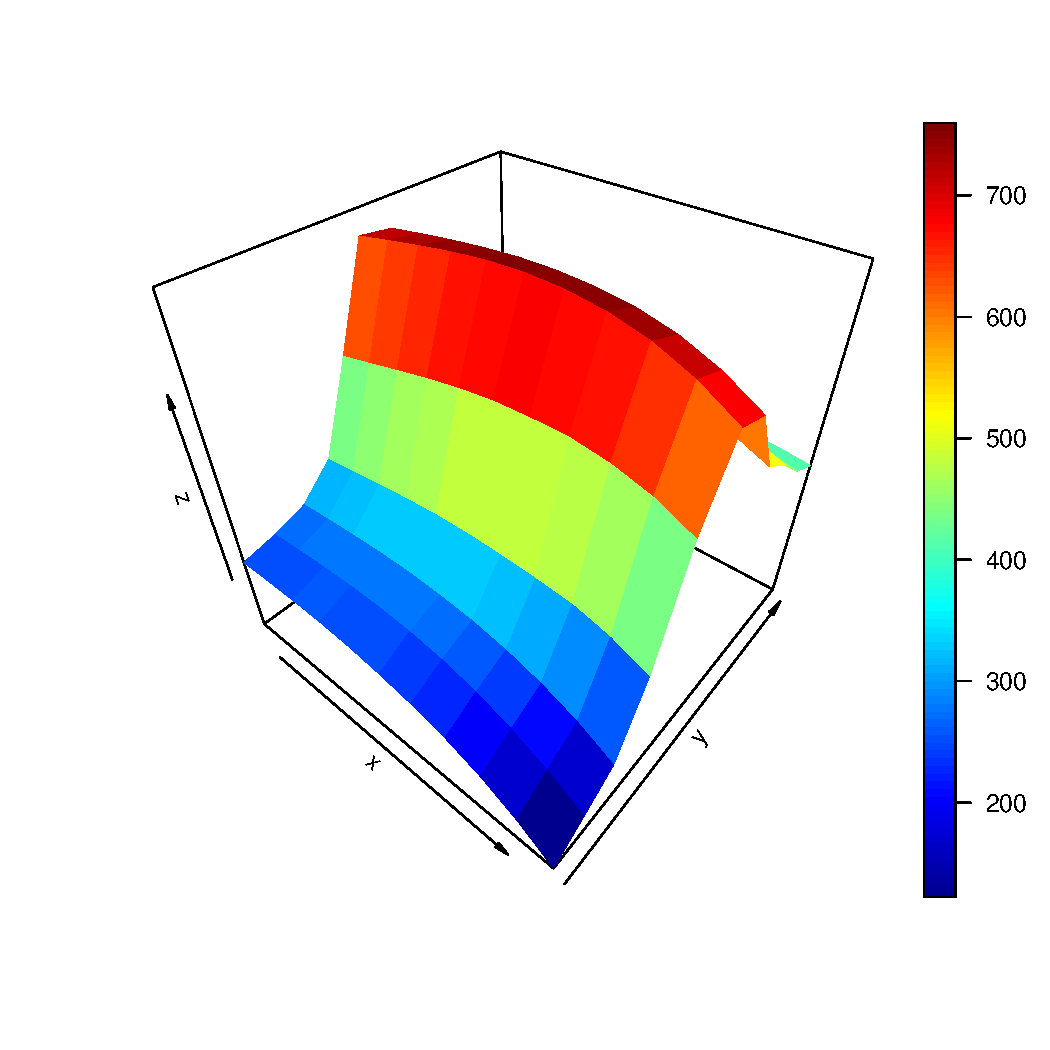
\includegraphics[width=\linewidth]{dtq_by100_by16.pdf}
\caption{DTQ by 100, by 16} \label{fig:e}
\end{subfigure}\hspace*{\fill}
\begin{subfigure}{0.48\textwidth}
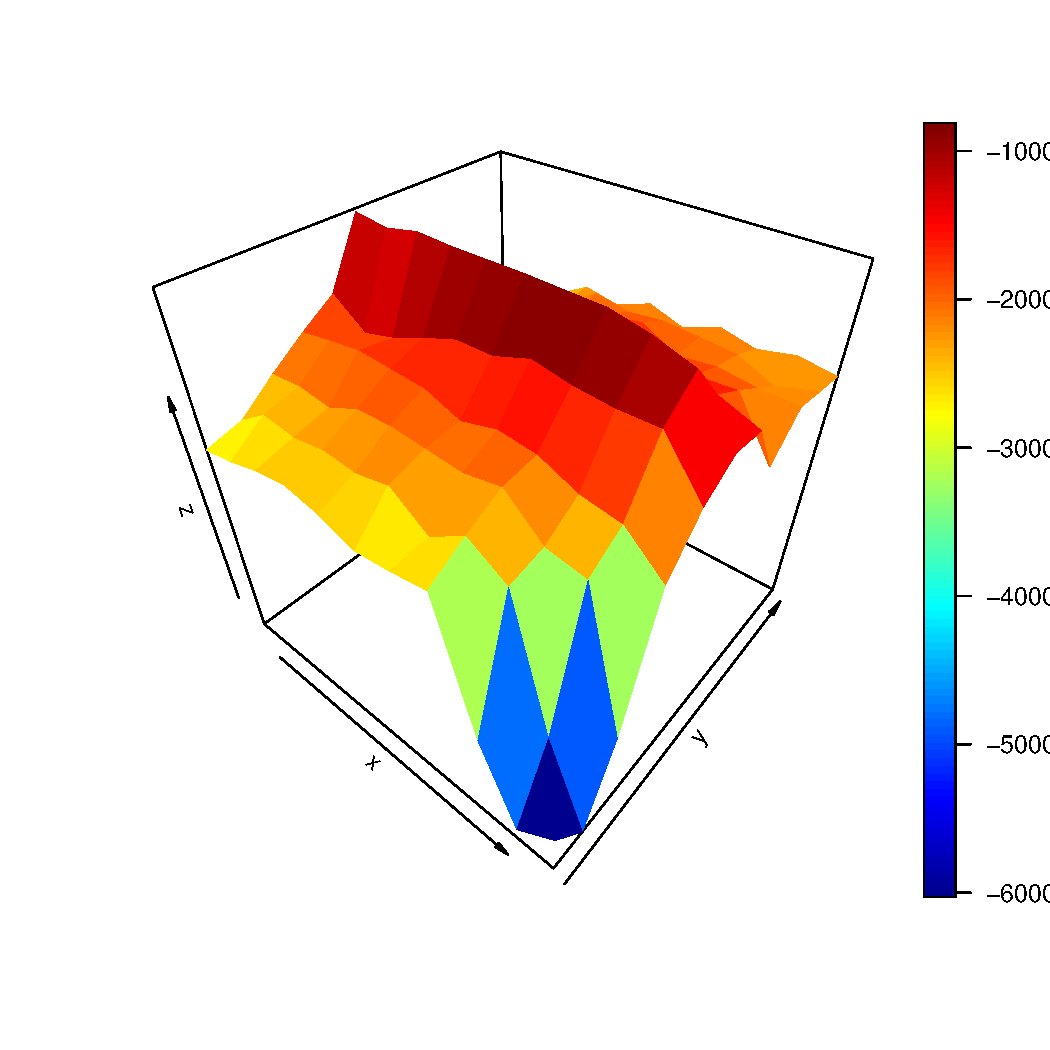
\includegraphics[width=\linewidth]{pomp_by100_by16.pdf}
\caption{POMP by 100, by 16} \label{fig:f}
\end{subfigure}

\caption{Likelihood surfaces for DTQ and POMP on the $\theta_2$ and $\theta_3$ grid}
\end{figure}

% \newpage

% \begin{figure}[H]
% \begin{subfigure}{0.48\textwidth}
% 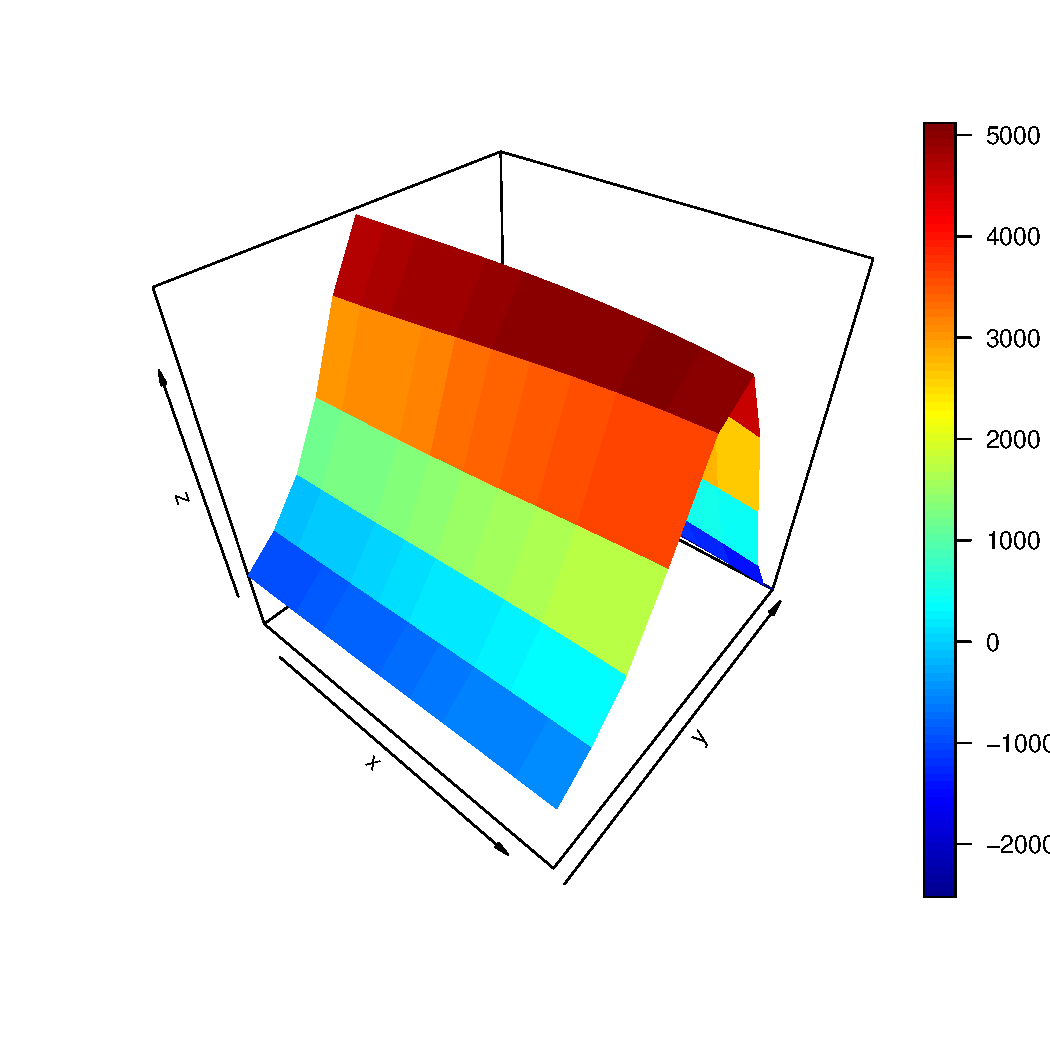
\includegraphics[width=\linewidth]{dtq_by10_by2.pdf}
% \caption{DTQ by 100, by 2} \label{fig:a}
% \end{subfigure}\hspace*{\fill}
% \begin{subfigure}{0.48\textwidth}
% 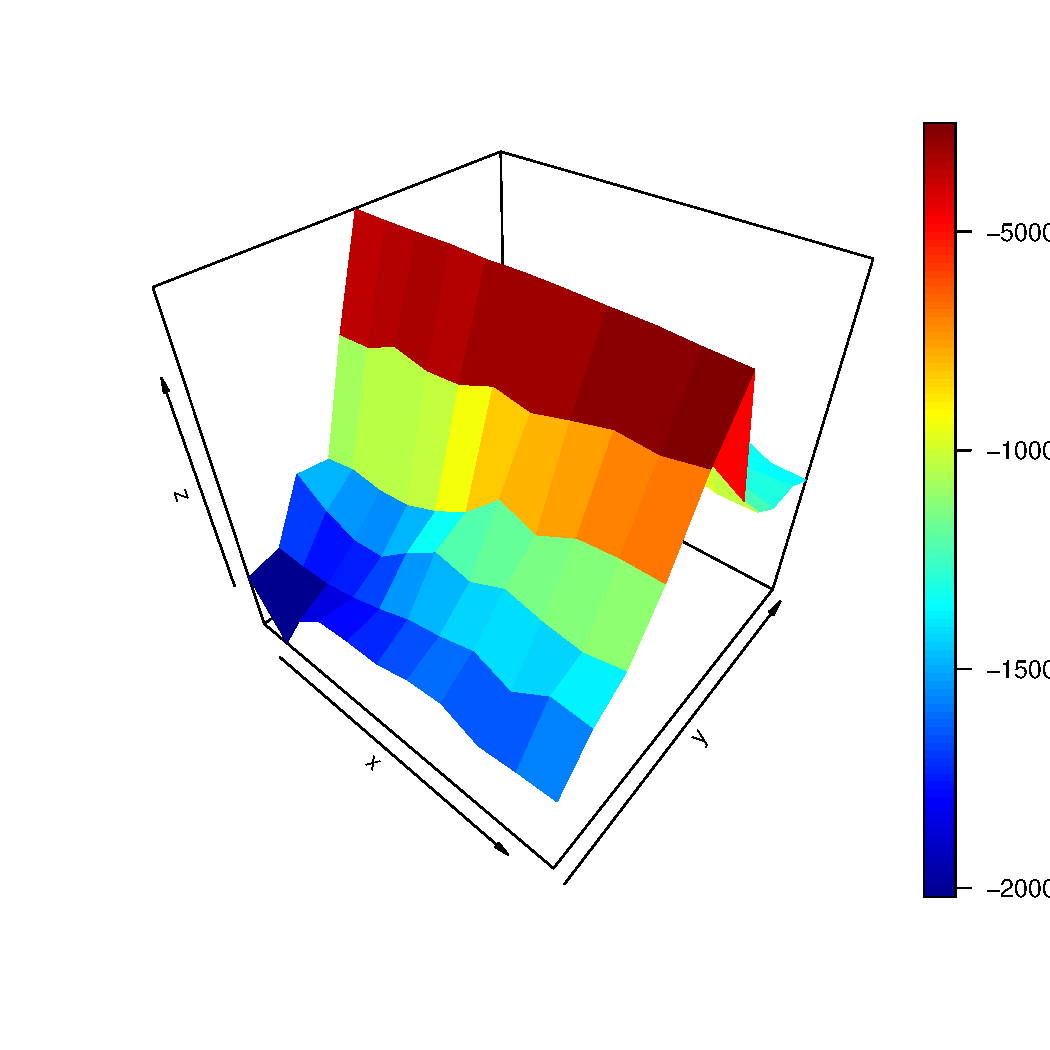
\includegraphics[width=\linewidth]{pomp_by10_by2.pdf}
% \caption{POMP by 100, by 2} \label{fig:b}
% \end{subfigure}


% \end{figure}

\newpage

TODO: Change this table with new MCMC code for POMP
MCMC steps = 2000, burnin steps = 100, measurement noise in $X_1$ and $X_2$ = $10^{-2}$

\begin{table}[h]
\centering
\begin{tabular}{lllllllll}
N particles & Min   & 1st Quad & Median & Mean  & 3rd Quad & Max   & Time            & Accept \% \\ \hline
10          & 5.835 & 6.386    & 6.386  & 6.522 & 6.386    & 7.550 & 37.124 + 3.032  & 0.0025\% \\
50          & 5.440 & 5.440    & 5.811  & 5.800 & 6.032    & 6.955 & 44.392 + 3.144  & 0.0045\% \\
100         & 5.309 & 5.499    & 5.617  & 5.741 & 5.925    & 6.785 & 44.736 + 3.024  & 0.006 \% \\
200         & 5.345 & 5.476    & 5.971  & 5.856 & 6.086    & 9.950 & 58.696 + 2.852  & 0.006\% \\
500         & 5.366 & 5.792    & 5.832  & 5.961 & 6.209    & 7.040 & 108.572 + 3.504 & 0.035\%            
\end{tabular}
\end{table}

\begin{table}[h]
\centering
\caption{POMP table of difference in means}
\begin{tabular}{|l|l|l|l|l|}
\hline
Difference Means & by 20       & by 50       & by 100      & by 200      \\ \hline
h by 1           & -0.05734111 & -0.06312163 & 0.02901005  & -0.2683111  \\ \hline
h by 2           & -0.05791024 & -0.1276239  & -0.373554   & 1.45994     \\ \hline
h by 3           & -0.06203916 & -0.0417083  & -0.2357552  & -0.1545804  \\ \hline
h by 4           & -0.08281177 & -0.06374529 & -0.2214498  & -0.4768346  \\ \hline
h by 5           & -0.0573322  & -0.05410928 & -0.02877429 & -0.1938626  \\ \hline
h by 6           &             &             & -0.06761619 & -0.1046286  \\ \hline
h by 7           &             &             & -0.1818962  & -0.03347735 \\ \hline
h by 8           &             &             & -0.05246908 & -0.2339528  \\ \hline
h by 9           &             &             & -0.2730433  & -0.1301727  \\ \hline
h by 10          &             &             & -0.02879612 & -0.06420363 \\ \hline
\end{tabular}
\end{table}

\begin{table}[h]
\centering
\caption{Rdtq2d - Table of difference in means}
\begin{tabular}{|l|l|l|l|l|}
\hline
Difference Means & by 20       & by 50 & by 100      & by 200      \\ \hline
h by 1           & 0.01799522  &       & 0.005835387 & 0.01591087  \\ \hline
h by 2           & -0.01703062 &       & -0.0628411  & -0.09772604 \\ \hline
h by 3           & 0.01168039  &       & -0.1564589  & -0.1512427  \\ \hline
h by 4           &             &       & -0.086696   & -0.1503922  \\ \hline
h by 5           &             &       & -0.09061449 & -0.166959   \\ \hline
h by 6           &             &       & -0.05866944 & -0.1651696  \\ \hline
h by 7           &             &       & -0.05619288 & -0.1609761  \\ \hline
h by 8           &             &       & -0.06385678 & -0.1642348  \\ \hline
h by 9           &             &       & -0.05940936 &             \\ \hline
h by 10          &             &       & -0.09577861 &             \\ \hline
\end{tabular}
\end{table}


\begin{table}[h]
\centering
\caption{POMP table of difference in modes}
\begin{tabular}{|l|l|l|l|l|}
\hline
Difference Modes & by 20       & by 50       & by 100      & by 200       \\ \hline
h by 1           & -0.0341092  & -0.03675144 & 0.04459498  & -0.2870469   \\ \hline
h by 2           & -0.04497344 & -0.02220465 & -0.01485807 & 2.482868     \\ \hline
h by 3           & -0.05712774 & -0.05975342 & -0.03467599 & -0.005828138 \\ \hline
h by 4           & -0.06649671 & -0.03845302 & -0.03029839 & -0.02734288  \\ \hline
h by 5           & -0.04263887 & -0.04431851 & -0.06616269 & -0.01583606  \\ \hline
h by 6           &             &             & -0.04524299 & 0.02920972   \\ \hline
h by 7           &             &             & -0.03962572 & -0.03218948  \\ \hline
h by 8           &             &             & -0.02710177 & -0.01554538  \\ \hline
h by 9           &             &             & -0.04130269 & -0.0286791   \\ \hline
h by 10          &             &             & -0.03013301 & -0.0237121   \\ \hline
\end{tabular}
\end{table}



\begin{table}[h]
\centering
\caption{Rdtq2d - Table of difference in modes}
\begin{tabular}{|l|l|l|l|l|}
\hline
Difference Modes & by 20       & by 50 & by 100      & by 200      \\ \hline
h by 1           & 0.007259653 &       & -0.01422478 & 0.1906643   \\ \hline
h by 2           & 0.0115566   &       & 0.02536292  & 0.0475644   \\ \hline
h by 3           & -0.01422478 &       & -0.02010194 & 0.01216831  \\ \hline
h by 4           &             &       & -0.04844341 & -0.03950003 \\ \hline
h by 5           &             &       & -0.05278264 & -0.02550886 \\ \hline
h by 6           &             &       & -0.04495679 & -0.02835948 \\ \hline
h by 7           &             &       & -0.04133994 & -0.01596862 \\ \hline
h by 8           &             &       & -0.04112844 & -0.02292278 \\ \hline
h by 9           &             &       & -0.03928337 &             \\ \hline
h by 10          &             &       & -0.03531033 &             \\ \hline
\end{tabular}
\end{table}


\begin{table}[h]
\centering
\caption{POMP table for acceptance ratios}
\begin{tabular}{|l|l|l|l|l|}
\hline
Acceptance Ratio & by 20 & by 50 & by 100 & by 200 \\ \hline
by 1             & 24.4  & 16.6  & 1.1    & 21.5   \\ \hline
by 2             &       & 19.7  & 46.6   & 41.1   \\ \hline
by 3             &       & 22.8  & 40     & 26     \\ \hline
by 4             &       & 15.5  & 36.9   & 55.7   \\ \hline
by 5             &       & 22.6  & 25.2   & 30.9   \\ \hline
\end{tabular}
\end{table}

\begin{table}[h]
\centering
\caption{Rdtq2d table for acceptance ratio}
\begin{tabular}{|l|l|l|l|l|}
\hline
Acceptance Ratio & by 20 & by 50 & by 100 & by 200 \\ \hline
by 1             & 28.5  & 33    & 37.6   & 52.9   \\ \hline
by 2             & 29.9  & 32    & 36.8   & 53.1   \\ \hline
by 3             &       & 32    & 47     & 52.5   \\ \hline
by 4             &       &       & 37.7   & 51     \\ \hline
by 5             &       &       & 37     & 50.3   \\ \hline
\end{tabular}
\end{table}

\begin{table}[h]
\centering
\caption{POMP table for time elapsed}
\begin{tabular}{|l|l|l|l|l|}
\hline
Elapsed time & by 20  & by 50  & by 100 & by 200 \\ \hline
by 1         & 95.541 & 42.380 & 24.946 & 16.118 \\ \hline
by 2         &        & 51.438 & 29.227 & 18.568 \\ \hline
by 3         &        & 60.414 & 33.762 & 20.685 \\ \hline
by 4         &        & 69.396 & 38.322 & 22.941 \\ \hline
by 5         &        & 78.251 & 42.895 & 25.025 \\ \hline
\end{tabular}
\end{table}

\begin{table}[h]
\centering
\caption{Rdtq2d table for time elapsed}
\begin{tabular}{|l|l|l|l|l|}
\hline
Elapsed time & by 20  & by 50  & by 100 & by 200 \\ \hline
by 1         & 0.143  & 0.151  & 0.143  & 0.138  \\ \hline
by 2         & 17.174 & 1.949  & 0.571  & 0.305  \\ \hline
by 3         &        & 67.011 & 12.370 & 3.073  \\ \hline
by 4         &        &        & 36.988 & 8.698  \\ \hline
by 5         &        &        & 98.264 & 17.898 \\ \hline
\end{tabular}
\end{table}



\end{document}